%----------------------------------------------------------------------------
%bb defines the bounding box for the pdf
%viewport defines the area of the pdf used
%in sidewaysfigure the last entry in bb moves the caption toward/away the pic
%in sidewaysfigure the second entry in bb moves the pic toward/away the caption
%----------------------------------------------------------------------------
\begin{figure}
\scalebox{0.8}[0.8]{
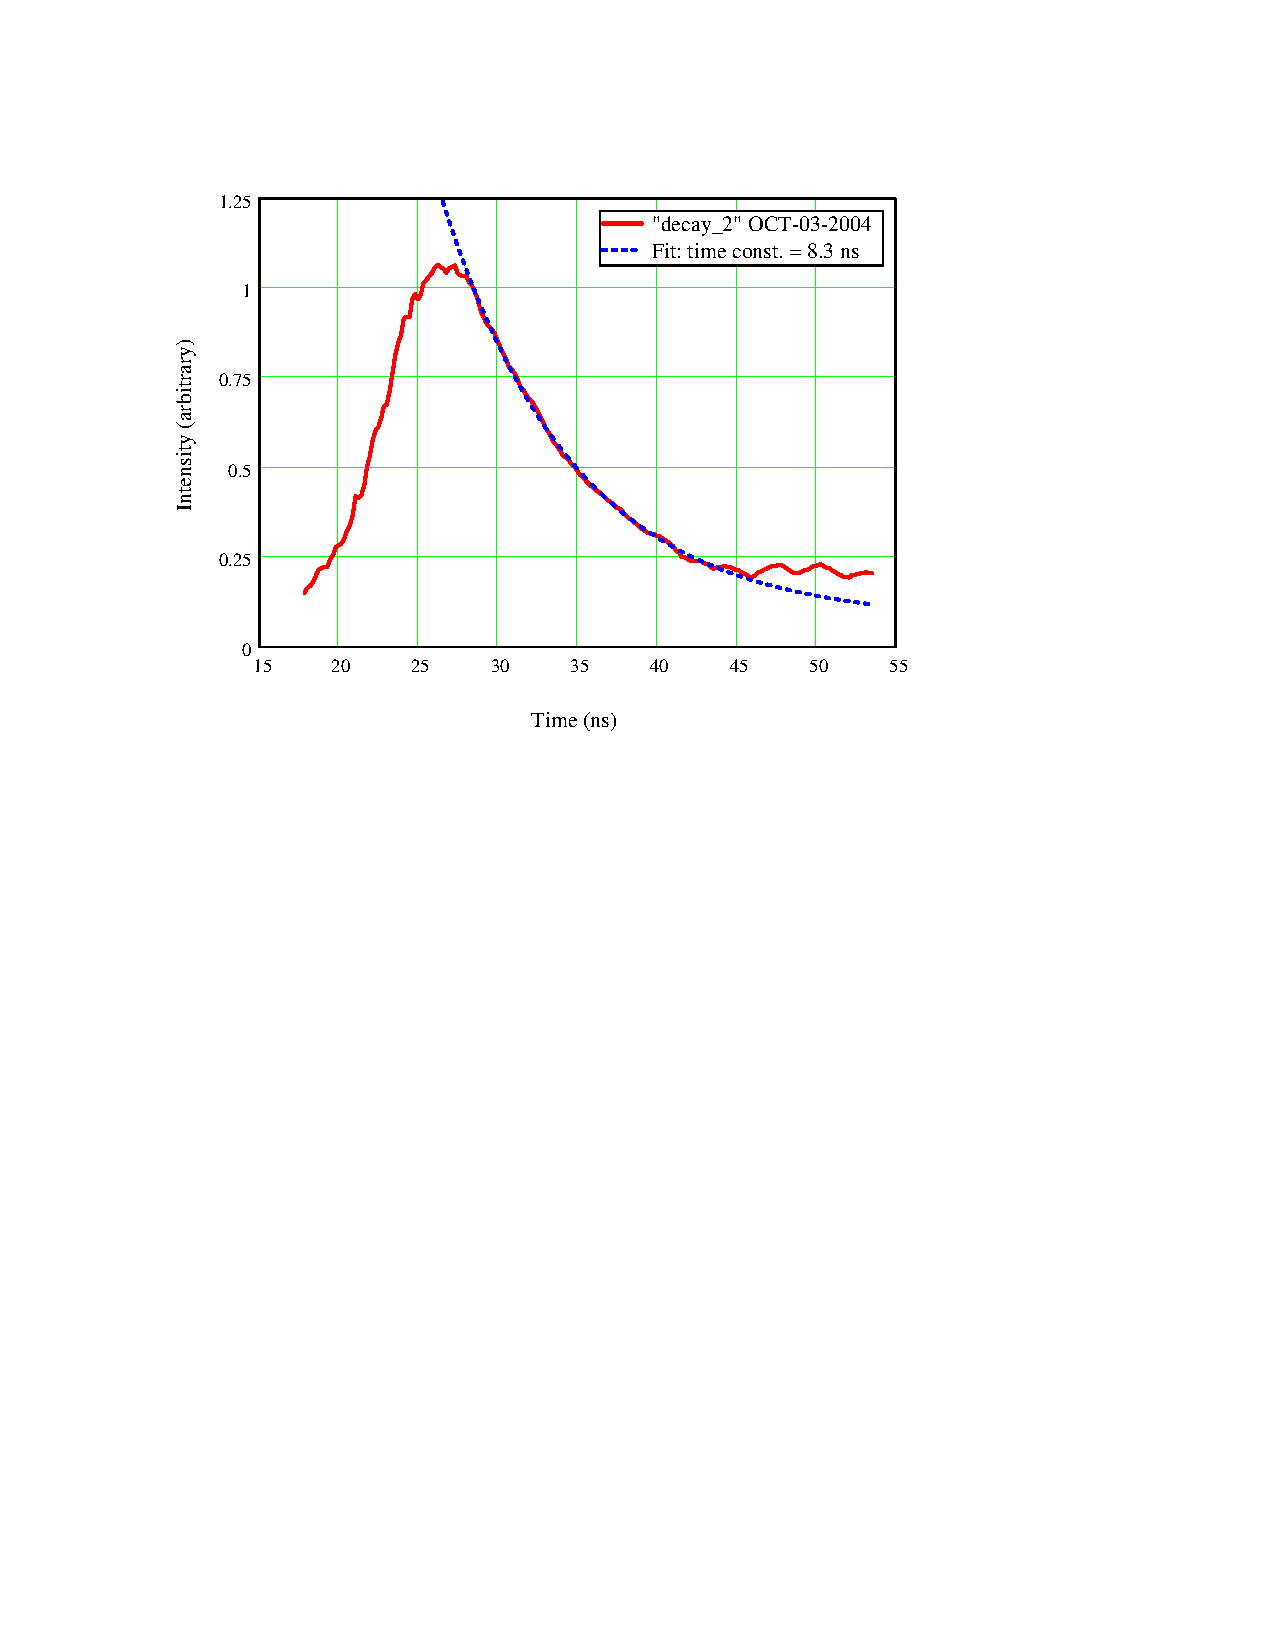
\includegraphics[bb=0 446 489 685]
{decay/decay.pdf}
}
\caption[Decay of 535.893 nm LIF line at 632.9 nm]{Decay of 535.893 nm LIF line at 632.9 nm (cell at $150^\circ$ F). The decay rate is inconsistent with the ideal calculation from Section \ref{LED section}; however, considering the likely contamination of the cell (see Figures \ref{iodine_potato} and \ref{baked_potato} and the associated discussion in Section \ref{res LIF section}}
\label{decay}
\end{figure}
%----------------------------------------------------------------------------
